%==============================================================================
% Chapitre 34 - Spin drift
%==============================================================================

\section{Introduction}

Lorsqu'un projectile est tiré sur une longue distance, son point d'impact
peut présenter une légère dérive latérale même en l'absence de vent.

Cette dérive est appelée dérive gyroscopique ou \emph{spin drift}.

Elle constitue une conséquence directe de la rotation du projectile et de son
comportement gyroscopique.

\begin{aretenir}

Le spin drift est une dérive latérale provoquée par la rotation du
projectile.

\end{aretenir}

\begin{figure}[htbp]
\centering
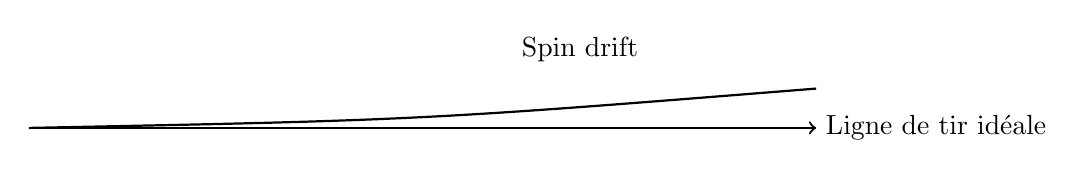
\begin{tikzpicture}

\draw[->,thick] (0,0) -- (10,0);
\node[right] at (10,0) {Ligne de tir idéale};

\draw[thick] (0,0) .. controls (5,0.1) .. (10,0.5);

\node at (7,1) {Spin drift};

\end{tikzpicture}
\caption{Illustration simplifiée de la dérive gyroscopique.}
\label{fig:spin_drift}
\end{figure}

\section{Observation du phénomène}

Le spin drift est généralement imperceptible aux courtes distances.

Cependant, lorsque la distance augmente :

\begin{itemize}
    \item le temps de vol augmente ;
    \item les effets gyroscopiques s'accumulent ;
    \item la dérive devient mesurable.
\end{itemize}

Il devient alors nécessaire d'en tenir compte dans les tirs de précision à
longue portée.

\section{Sens de la dérive}

Le sens du spin drift dépend du sens de rotation imposé par les rayures.

Pour un canon à rayures droites :

\begin{itemize}
    \item le projectile tourne dans le sens horaire vu depuis le tireur ;
    \item la dérive apparaît généralement vers la droite.
\end{itemize}

Pour un canon à rayures gauches :

\begin{itemize}
    \item la rotation est inversée ;
    \item la dérive apparaît généralement vers la gauche.
\end{itemize}

\section{Une idée fausse fréquente}

Le spin drift n'est pas causé par un effet centrifuge.

Le projectile ne « visse » pas dans l'air.

Cette explication est incorrecte.

L'origine réelle est beaucoup plus subtile et implique le comportement
gyroscopique du projectile.

\section{Lien avec la précession}

Nous avons vu qu'un projectile en rotation répond aux moments aérodynamiques
par un mouvement de précession.

Pendant son vol :

\begin{itemize}
    \item la gravité courbe progressivement la trajectoire ;
    \item l'axe du projectile cherche à suivre cette évolution ;
    \item des moments aérodynamiques apparaissent.
\end{itemize}

La réponse gyroscopique du projectile produit alors une petite composante
latérale.

\section{Le phénomène de yaw of repose}

Au cours du vol, le projectile adopte progressivement une très faible
inclinaison moyenne.

Cette inclinaison est appelée \emph{yaw of repose}.

Elle est extrêmement faible :

\begin{itemize}
    \item souvent de l'ordre de quelques minutes d'angle ;
    \item parfois moins.
\end{itemize}

Pourtant, elle suffit à générer une force latérale mesurable.

\section{Origine de la force latérale}

Le yaw of repose produit une légère asymétrie aérodynamique.

Cette asymétrie génère :

\begin{itemize}
    \item une faible portance latérale ;
    \item une dérive progressive ;
    \item un déplacement du point d'impact.
\end{itemize}

Le spin drift résulte principalement de ce mécanisme.

\section{Accumulation pendant le vol}

La dérive gyroscopique agit pendant toute la durée du vol.

Même si la force latérale reste faible :

\begin{itemize}
    \item le temps de vol est important ;
    \item l'effet s'accumule ;
    \item l'écart devient visible.
\end{itemize}

\section{Influence de la distance}

Le spin drift augmente généralement avec :

\begin{itemize}
    \item la distance ;
    \item le temps de vol.
\end{itemize}

C'est pourquoi il est principalement étudié pour les tirs longue portée.

\section{Influence de la vitesse}

La vitesse influence le phénomène de plusieurs manières :

\begin{itemize}
    \item elle modifie le temps de vol ;
    \item elle modifie les forces aérodynamiques ;
    \item elle influence la stabilité gyroscopique.
\end{itemize}

Le comportement exact dépend du projectile considéré.

\section{Influence du pas de rayure}

Le pas de rayure détermine la vitesse de rotation.

Il influence donc indirectement :

\begin{itemize}
    \item le comportement gyroscopique ;
    \item le yaw of repose ;
    \item le spin drift.
\end{itemize}

\section{Ordres de grandeur}

À courte distance :

\begin{itemize}
    \item l'effet est généralement négligeable.
\end{itemize}

À longue distance :

\begin{itemize}
    \item quelques centimètres ;
    \item plusieurs dizaines de centimètres ;
    \item voire davantage selon les conditions.
\end{itemize}

Le phénomène devient alors comparable à d'autres corrections importantes.

\section{Spin drift et vent}

Le spin drift ne doit pas être confondu avec la dérive due au vent.

Les deux effets :

\begin{itemize}
    \item possèdent des causes différentes ;
    \item peuvent agir simultanément ;
    \item doivent être corrigés séparément.
\end{itemize}

\section{Spin drift et Coriolis}

Le spin drift ne doit pas non plus être confondu avec :

\begin{itemize}
    \item l'effet Coriolis ;
    \item l'effet Eötvös ;
    \item les effets géophysiques.
\end{itemize}

Ces phénomènes possèdent des origines totalement différentes.

\section{Importance pratique}

Dans les tirs courants :

\begin{itemize}
    \item le spin drift est souvent négligeable.
\end{itemize}

Dans les tirs de précision à grande distance :

\begin{itemize}
    \item il peut devenir nécessaire de le corriger ;
    \item les calculateurs balistiques le prennent généralement en compte.
\end{itemize}

\section{Spin drift et simulation}

Les modèles simples ignorent souvent le spin drift.

Les modèles avancés peuvent le reproduire.

Il apparaît naturellement dans les modèles :

\begin{itemize}
    \item 5DOF ;
    \item 6DOF ;
    \item gyroscopiques complets.
\end{itemize}

\begin{simulation}

La reproduction correcte du spin drift constitue un indicateur important de
la qualité d'un modèle balistique avancé.

\end{simulation}

\section{Synthèse des phénomènes gyroscopiques}

Nous avons maintenant étudié :

\begin{itemize}
    \item la stabilisation gyroscopique ;
    \item la précession ;
    \item la nutation ;
    \item le spin drift.
\end{itemize}

Ces phénomènes sont intimement liés et résultent tous de la rotation du
projectile.

\section{Vers les critères de stabilité}

Nous savons désormais pourquoi un projectile tourne et comment cette rotation
influence son comportement.

Une question importante demeure :

\begin{quote}
Comment déterminer quantitativement si un projectile est suffisamment
stabilisé ?
\end{quote}

Cette question conduit aux critères et facteurs de stabilité.

\section{À retenir}

\begin{aretenir}

\begin{itemize}
    \item Le spin drift est une dérive latérale liée à la rotation du
          projectile.
    \item Il résulte du comportement gyroscopique du projectile.
    \item Il dépend du sens des rayures.
    \item Il devient significatif aux longues distances.
    \item Il ne doit pas être confondu avec le vent ou l'effet Coriolis.
\end{itemize}

\end{aretenir}
